%%%%%%%%%%%%%%%%%%%%%%%%%%%%%%%%%%%%%%%%%%%%%%%%%%%%%%%
%%%%               FORMATTING AND COLORING         %%%%
%%%%%%%%%%%%%%%%%%%%%%%%%%%%%%%%%%%%%%%%%%%%%%%%%%%%%%%
\documentclass[xcolor=dvipsnames]{beamer}
%\RequirePackage[2017/04/15]{latexrelease}
\definecolor{Fuchsia}{HTML}{000000}
\definecolor{SlateGrey}{HTML}{F7BF0A}


%\definecolor{LightGrey}{HTML}{666666}

\colorlet{accent}{Fuchsia}
\colorlet{emphasis}{SlateGrey}

\usepackage{caption}

\usetheme{CambridgeUS}
\useinnertheme{rectangles}
\useoutertheme{infolines}
\usepackage{xcolor}
\usepackage{listings}


%%%%%%%%%%%%%%%%%%%%%%%%%%%%%%%%%%%%%%%%%%%%%
%this adds in the circles to the right of background
%%%%%%%%%%%%%%%%%%%%%%%%%%%%%%%%%%%%%%%%%%%%%
\makeatletter
\def\insertsubsectionnavigationhorizontal#1#2#3{%
    \hbox to #1{{%
        \usebeamerfont{subsection in head/foot}\usebeamercolor[fg]{subsection in head/foot}
        \beamer@currentsubsection=0%
        \def\sectionentry##1##2##3##4##5{}%
        \def\slideentry##1##2##3##4##5##6{\ifnum##6=\c@part\ifnum##1=\c@section%
      \ifnum##2>\beamer@currentsubsection%
      \box\beamer@sectionbox\hskip1.875ex plus1fill%
            \hbox to 0pt{%
                    \global\beamer@section@min@dim\beamer@tempdim
                        \beamer@link(##4){%
                            \usebeamerfont{mini frame}%
                            \ifnum\c@section=##1%
                                \ifnum\c@subsection=##2%
                                    \usebeamercolor[fg]{mini frame}%
                                    \ifnum\c@subsectionslide=##3%
                                        \usebeamertemplate{mini frame}%\beamer@minislidehilight%
                                    \else%
                                        \usebeamertemplate{mini frame in current subsection}%\beamer@minisliderowhilight%
                                    \fi%
                                \else%
                                    \usebeamercolor{mini frame}%
                                    %\color{fg!50!bg}%
                                    \usebeamertemplate{mini frame in other subsection}%\beamer@minislide%
                                \fi%
                            \else%
                                \usebeamercolor{mini frame}%
                                                                %\color{fg!50!bg}%
                                \usebeamertemplate{mini frame in other subsection}%\beamer@minislide%
                            \fi%
                        }%
                \hskip-10cm plus 1fil%
            }%
            \fi\fi\fi\ignorespaces
        }%
        #2\hskip.3cm\setbox\beamer@sectionbox=\hbox{}%
        \hskip-1.875ex plus-1fill\dohead%
        \box\beamer@sectionbox\hfil\hskip.3cm%
        #3
    }}
}

\setbeamertemplate{footline}%{infolines theme}
{
  \leavevmode%
  \hbox{%
  \begin{beamercolorbox}[wd=.333333\paperwidth,ht=2.25ex,dp=1ex,center]{author in head/foot}%
    \usebeamerfont{author in head/foot}\insertshortauthor\expandafter\beamer@ifempty\expandafter{\beamer@shortinstitute}{}{~~(\insertshortinstitute)}
  \end{beamercolorbox}%
  \begin{beamercolorbox}[wd=.333333\paperwidth,ht=2.25ex,dp=1ex,center]{title in head/foot}%
    \usebeamerfont{title in head/foot}\insertshorttitle
  \end{beamercolorbox}%
  \begin{beamercolorbox}[wd=.333333\paperwidth,ht=2.25ex,dp=1ex,right]{date in head/foot}%
    \usebeamerfont{date in head/foot} %\insertshortdate{} % remove the date from each slide 
    % could insert text here to make it display in the footer 
    \hspace*{2em}
    \insertframenumber{} / \inserttotalframenumber\hspace*{2ex} 
  \end{beamercolorbox}}%
  \vskip0pt%
}
\makeatother

\setbeamertemplate{headline}
{
  \leavevmode%
  \hbox{%
  \begin{beamercolorbox}[wd=.5\paperwidth,ht=2.65ex,dp=1.5ex,right]{section in head/foot}%
    \usebeamerfont{section in head/foot}\bfseries\insertsectionhead\hspace*{2ex}
  \end{beamercolorbox}%
  \begin{beamercolorbox}[wd=.5\paperwidth,ht=2.65ex,dp=1.5ex,left]{subsection in head/foot}%
    \usebeamerfont{subsection in head/foot}\setbeamercolor{section in head/foot}{fg=Fuchsia!125,bg=white}
    \vspace*{.01cm}\insertsubsectionnavigationhorizontal{.5cm}{\hskip-.1cm}{}
  \end{beamercolorbox}}%
  \vskip0pt%
}
% gets rid of navigation symbols
\setbeamertemplate{navigation symbols}{}
% add figures numbering
\setbeamertemplate{caption}[numbered]

\setbeamercolor{frametitle}{fg=Fuchsia,bg=SlateGrey}
\setbeamercolor{section in head/foot}{fg= SlateGrey!75, bg=Fuchsia}
\setbeamercolor{title in head/foot}{fg=Fuchsia, bg=SlateGrey!45}
\setbeamercolor{subsection in head/foot}{fg=Fuchsia, bg=Black!15}
\setbeamercolor{author in head/foot}{bg=SlateGrey, fg=SlateGrey}
\setbeamercolor{date in head/foot}{fg=Fuchsia, bg =SlateGrey!15}
\setbeamercolor{structure}{fg=Fuchsia, bg= SlateGrey}
\setbeamercolor{frametitle}{fg= Fuchsia}
\setbeamercolor{title}{fg=Fuchsia}
\setbeamercolor*{palette tertiary}{bg=Fuchsia}
\setbeamercolor{section in sidebar}{fg=Fuchsia}
\setbeamercolor{titlelike}{bg =SlateGrey}



\newenvironment{colorframe}[2][]{%
\setbeamercolor{background canvas}{bg=#1}
\begin{frame}\frametitle{#2}}
{\end{frame}}
%%%%%%%%%%%%%%%%%%%%%%%%%%%%%%%%%%%%%%%%%%%%%%%%%%%
% End of customizing the theme layout and colors 
%%%%%%%%%%%%%%%%%%%%%%%%%%%%%%%%%%%%%%%%%%%%%%%%%%%
\usepackage{comment}
\usepackage[T1]{fontenc}
\usepackage[default]{lato}
\usepackage[english]{babel}
\usepackage[utf8x]{inputenc}
\usepackage{pslatex}
\usepackage{fontawesome}
\usepackage{animate}

\usepackage{xmpmulti}

\usepackage{subcaption}
\captionsetup{compatibility=false}
%%%%%%%%%%%%%%%%%%%%%%%%%%%%%%%%%%%%%%%%%%%%%%%%%%%%%%%
%%%%%%%%%%%%%%%%%%%%%%%%%%%%%%%%%%%%%%%%%%%%%%%%%%%%%%%
%%%%          Beginning of the slide deck          %%%%
%%%%%%%%%%%%%%%%%%%%%%%%%%%%%%%%%%%%%%%%%%%%%%%%%%%%%%%
%%%%%%%%%%%%%%%%%%%%%%%%%%%%%%%%%%%%%%%%%%%%%%%%%%%%%%%



%changing the color of bullet points 
%\newenvironment{a2env}{\only{\setbeamercolor{local structure}{fg=climateChange}}}{}
%\newenvironment{rtenv}{\only{\setbeamercolor{local structure}{fg=recentTrends}}}{}
%%%%%%%%%%%%
%title page%
%%%%%%%%%%%%
\title[UCF Math Club Meeting 2]{Learning Some LaTeX}
\author{}
\institute{University of Central Florida}
\date{\scriptsize{September 14th, 2018}}

\begin{document}
\begin{frame}
  \titlepage
  \vfill
 % 
\includegraphics[width=.1\linewidth]{University-of-Central-Florida-logo-Black.png} \hfill %
\includegraphics[width=.11\linewidth]{Harvard_Forest_logo_high_res.jpg}
\end{frame}

\section{House Keeping}
\subsection{}

\begin{frame}{Dues, T-shirts, and JMM}
Dues are \$20. They are not mandatory. \newline
If you decide to pay dues, you get a t-shirt,  are eligible to apply for JMM travel assistance, and are eligible to vote in officer elections in April.\newline

\end{frame}

\begin{colorframe}[black]{T-Shirt Design}

\begin{center}

\begin{columns}
    \begin{column}{0.48\textwidth}
     
\includegraphics[height = \linewidth]{tshirtbackdarkerblack.png}
    \end{column}
    \begin{column}{0.48\textwidth}
     
\includegraphics[width = \linewidth]{UCF_CMS_LOGO_tshirttrans.png}
    \end{column}
\end{columns}

\end{center}
\end{colorframe}

\begin{frame}{Joint Meeting in Mathematics (JMM) Information} 

\end{frame}

\begin{frame}{Grad School PSA (last chance)}
Applications due in December, but it is usually a good idea to have them done before the deadlines. A grad school application normally consists of the following, 
\begin{itemize}
\item Personal Statement
\item Transcripts from past institutions
\item GRE scores
\begin{itemize}
\item GRE 
\item \textbf{GRE Math Subject test }(for those of you pursuing Mathematics Phd) 

\end{itemize}
\end{itemize}
\end{frame}

\section{LaTeX}
\subsection{}

\begin{frame}{What is LaTeX?}

\centering \LaTeX is a document preparation system created in 1983. 

\vfill
\small{"\LaTeX is widely used in academia for the communication and publication of scientific documents in many fields, including mathematics, statistics, computer science, engineering, chemistry, physics, economics, linguistics, quantitative psychology, philosophy, and political science." - Wikipedia}

\vfill 
\centering \textbf{lay-tech or lah-tech but definitely not latex}

\end{frame}

\begin{frame}{Why would you use LaTeX?}
\begin{itemize}
\item You want to focus on content only,
\item You want to produce a heavily customized document, or 
\item You need to type up mathematics symbols in a report or assignment. 
\end{itemize}


\centering 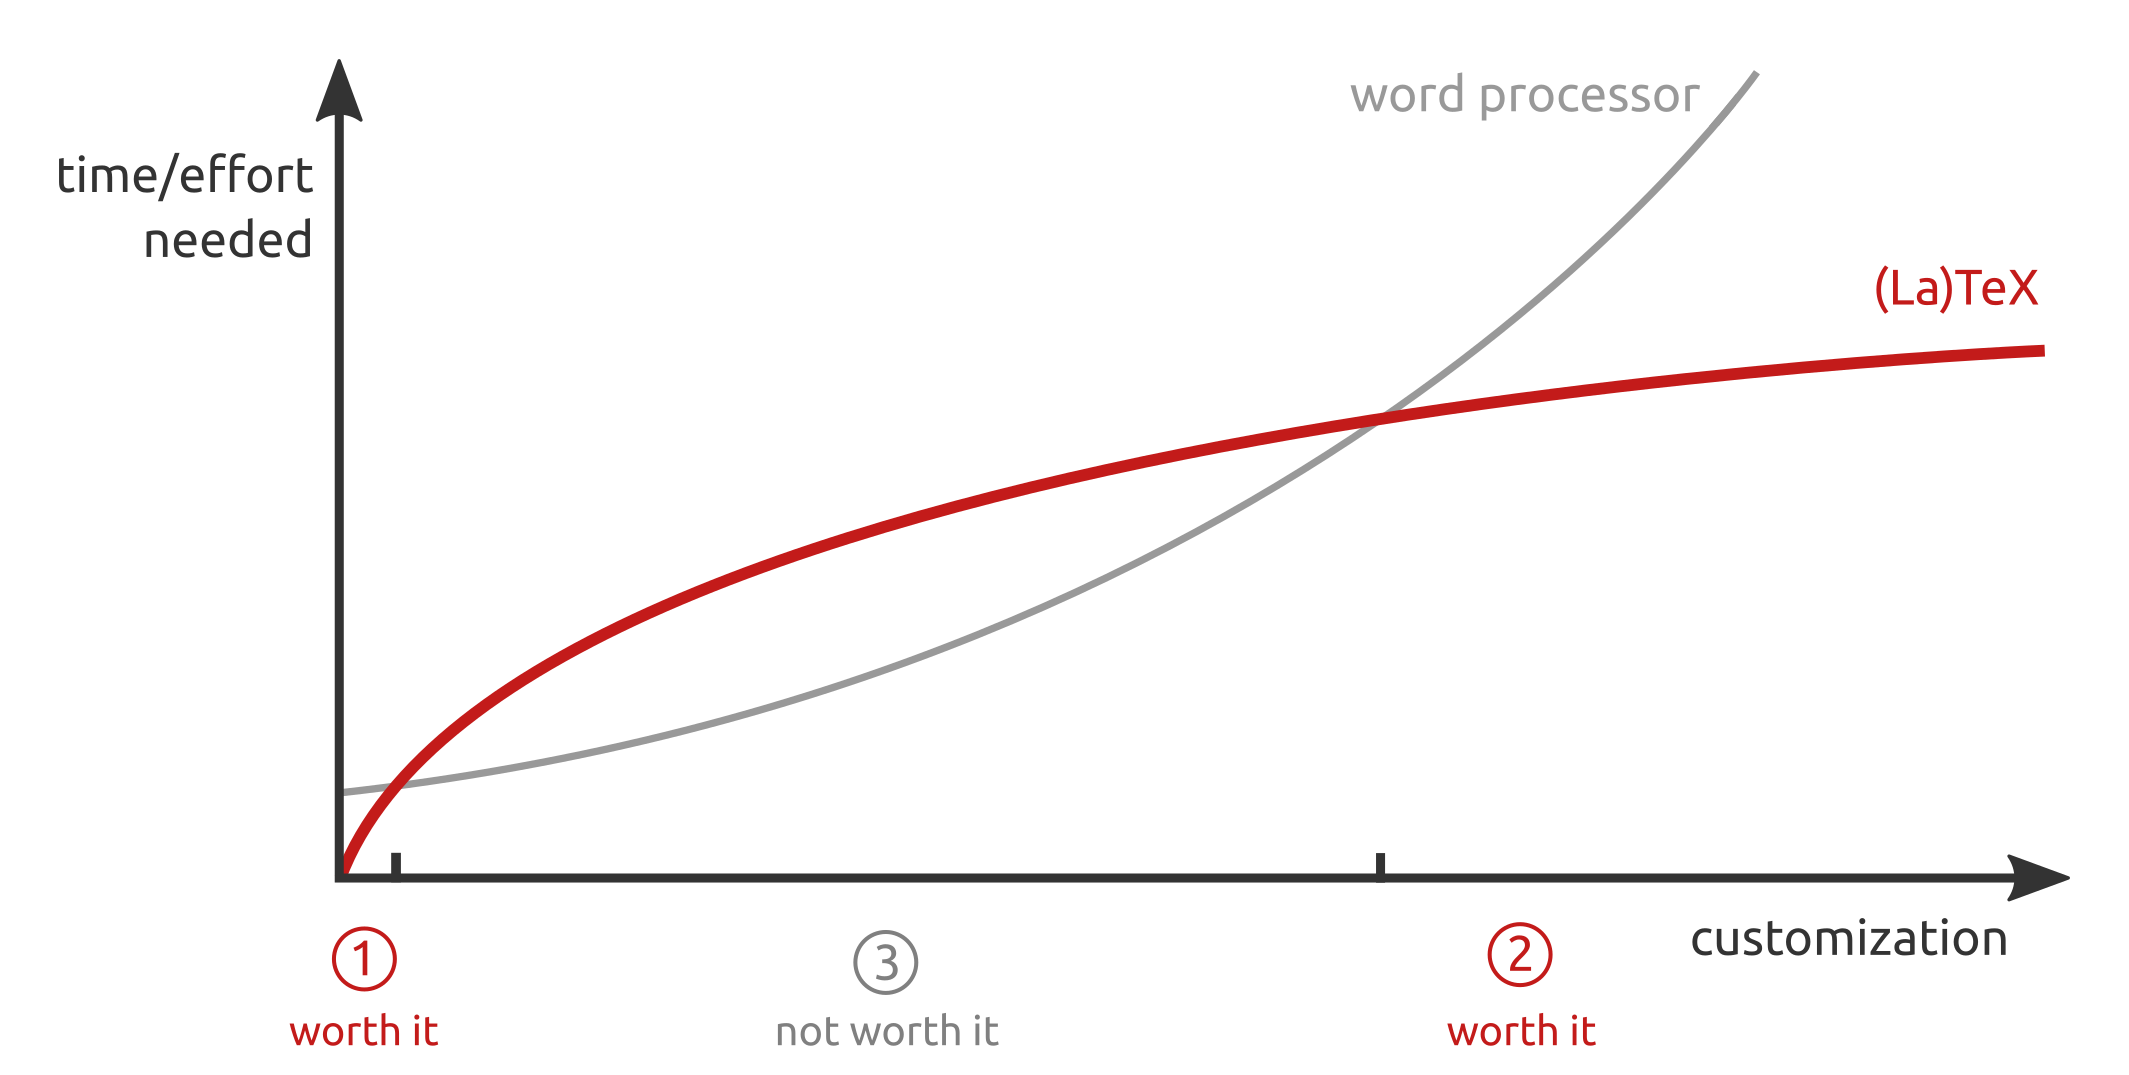
\includegraphics[width =.8\linewidth]{timeVeffort.png}

\end{frame} 

\begin{frame}{Some Examples} 

\centering \Large \textbf{\color{blue} https://github.com/waldmannly/Latex-Templates}

\vfill
\begin{center}
\centering Online editors: Overleaf/ShareTeX 


\centering Local editors: TeX Maker and MikTeX
\end{center}
\end{frame}

\begin{frame}{Some Basics} 
\lstset{language=TeX}
\scriptsize\lstinputlisting{simplefile.tex}
\end{frame}

\begin{frame}{Go Forth and Practice} 

You should either try to convert your resume or type up a homework assignment. The officers (, Google,) and I will be available until the end of the meeting for question about syntax or the weird \LaTeX quarks (try to put a space in an equation and see what happens). 

\vfill 

Also check out the templates hosted on Overleaf. 

\end{frame}



\end{document}

